% Auto-generated by figures/generate_paper_assets.py

% === Figure 1: Relation/COCO Pareto ===
\begin{figure*}[t]
    \centering
    % Auto-generated by figures/generate_paper_assets.py
\begin{tikzpicture}[font=\footnotesize]
\draw[->] (0,0) -- (7.05,0) node[right] {Relation accuracy};
\draw[->] (0,0) -- (0,4.25) node[above] {COCO I2T R@1};
\draw (0.40,0.04) -- (0.40,-0.04) node[below] {0.65};
\draw (2.40,0.04) -- (2.40,-0.04) node[below] {0.70};
\draw (4.40,0.04) -- (4.40,-0.04) node[below] {0.75};
\draw (6.40,0.04) -- (6.40,-0.04) node[below] {0.80};
\draw (0.04,0.50) -- (-0.04,0.50) node[left] {0.40};
\draw (0.04,1.33) -- (-0.04,1.33) node[left] {0.50};
\draw (0.04,2.17) -- (-0.04,2.17) node[left] {0.60};
\draw (0.04,3.00) -- (-0.04,3.00) node[left] {0.70};
\draw (0.04,3.83) -- (-0.04,3.83) node[left] {0.80};
\draw[densely dashed,gray] (2.22,0) -- (2.22,4.00);
\draw[densely dashed,gray] (0,3.00) -- (6.80,3.00);
\node[gray,anchor=south west] at (2.27,0.05) {R005 relation};
\node[gray,anchor=south east] at (6.75,3.05) {COCO gate};
\node[circle,draw=black,fill=black,inner sep=1.8pt] (R003) at (0.66,3.83) {};
\node[anchor=west] at (0.74,3.93) {R003};
\node[circle,draw=gray,fill=gray,inner sep=1.8pt] (R005) at (2.22,3.66) {};
\node[anchor=west] at (2.30,3.76) {R005};
\node[rectangle,draw=red!75!black,fill=red!75!black,inner sep=1.8pt] (R011) at (4.35,0.43) {};
\node[anchor=west] at (4.43,0.53) {R011};
\node[rectangle,draw=red!75!black,fill=red!75!black,inner sep=1.8pt] (R014) at (3.73,0.59) {};
\node[circle,draw=blue!75!black,fill=blue!75!black,inner sep=1.8pt] (R019) at (5.19,3.16) {};
\node[circle,draw=blue!75!black,fill=blue!75!black,inner sep=1.8pt] (R023) at (6.09,2.85) {};
\node[circle,draw=gray,fill=gray,inner sep=1.8pt] (R024) at (1.34,3.83) {};
\node[circle,draw=blue!75!black,fill=blue!75!black,inner sep=2.3pt] (R028) at (5.34,3.28) {};
\node[anchor=east] at (5.26,3.38) {R028};
\node[circle,draw=blue!75!black,fill=blue!75!black,inner sep=1.8pt] (R029) at (5.32,3.23) {};
\node[circle,draw=blue!75!black,fill=blue!75!black,inner sep=1.8pt] (R031) at (5.64,3.22) {};
\node[circle,draw=blue!75!black,fill=blue!75!black,inner sep=1.8pt] (R032) at (5.62,2.78) {};
\node[diamond,draw=orange!85!black,fill=orange!85!black,inner sep=1.8pt] (R033) at (5.70,0.28) {};
\node[anchor=east] at (5.62,0.38) {R033};
\node[circle,draw=cyan!60!black,fill=cyan!60!black,inner sep=1.8pt] (R035) at (5.61,3.11) {};
\node[circle,draw=cyan!60!black,fill=cyan!60!black,inner sep=1.8pt] (R036) at (5.60,2.85) {};
\node[circle,draw=cyan!60!black,fill=cyan!60!black,inner sep=1.8pt] (R037) at (5.66,3.12) {};
\node[circle,draw=cyan!60!black,fill=cyan!60!black,inner sep=1.8pt] (R038) at (5.34,3.36) {};
\node[anchor=east] at (5.26,3.46) {R038};
\node[circle,draw=cyan!60!black,fill=cyan!60!black,inner sep=1.8pt] (R039) at (5.58,2.95) {};
\node[diamond,draw=orange!85!black,fill=orange!85!black,inner sep=1.8pt] (R040) at (5.49,1.18) {};
\node[circle,draw=purple!75!black,fill=purple!75!black,inner sep=1.8pt] (R043) at (4.17,3.30) {};
\node[anchor=west] at (4.25,3.40) {R043};
\draw[dashed,thick,black!55] (1.34,3.83) -- (2.22,3.66) -- (5.34,3.36) -- (6.09,2.85);
\node[black!60,anchor=west] at (4.65,2.70) {evaluated frontier};
\node[anchor=west] at (0.15,4.05) {\tikz\node[circle,draw=blue!75!black,fill=blue!75!black,inner sep=1.5pt]{}; RRB};
\node[anchor=west] at (1.55,4.05) {\tikz\node[rectangle,draw=red!75!black,fill=red!75!black,inner sep=1.4pt]{}; hard token};
\node[anchor=west] at (3.25,4.05) {\tikz\node[diamond,draw=orange!85!black,fill=orange!85!black,inner sep=1.5pt]{}; no-channel};
\node[anchor=west] at (5.25,4.05) {\tikz\node[circle,draw=cyan!60!black,fill=cyan!60!black,inner sep=1.5pt]{}; anchor-20};
\end{tikzpicture}

    \caption{Relation accuracy versus COCO image-to-text retrieval for key evaluated systems. Hard-token controls replace the pretrained embedding path with a bottlenecked representation, while no-channel controls use a residual path without the multi-channel bottleneck. Standard PEFT baselines such as LoRA and text-only tuning were not evaluated in this ablation study, which focuses on the architectural impact of the RRB bottleneck.}
    \label{fig:relation_coco}
\end{figure*}

% === Figure 2: Seed and anchoring summary ===
\begin{figure}[t]
    \centering
    % Auto-generated by figures/generate_paper_assets.py
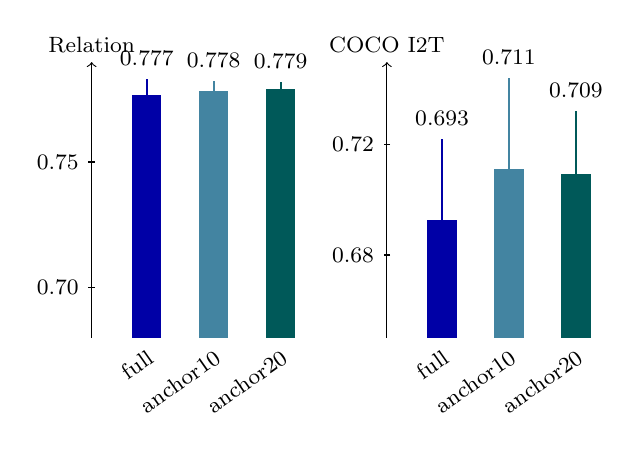
\begin{tikzpicture}[font=\footnotesize]
\draw[->] (0,0) -- (0,3.50) node[above] {Relation};
\draw[->] (3.75,0) -- (3.75,3.50) node[above] {COCO I2T};
\draw (0.04,0.64) -- (-0.04,0.64) node[left] {0.70};
\draw (0.04,2.23) -- (-0.04,2.23) node[left] {0.75};
\draw (3.79,1.05) -- (3.71,1.05) node[left] {0.68};
\draw (3.79,2.45) -- (3.71,2.45) node[left] {0.72};
\draw[fill=blue!65!black,draw=blue!65!black] (0.52,0) rectangle (0.88,3.08);
\draw[blue!65!black,thick] (0.70,2.88) -- (0.70,3.28);
\node[rotate=35,anchor=east] at (0.85,-0.15) {full};
\node[above] at (0.70,3.33) {0.777};
\draw[fill=blue!65!black,draw=blue!65!black] (4.27,0) rectangle (4.63,1.49);
\draw[blue!65!black,thick] (4.45,0.47) -- (4.45,2.52);
\node[rotate=35,anchor=east] at (4.60,-0.15) {full};
\node[above] at (4.45,2.57) {0.693};
\draw[fill=cyan!60!black,draw=cyan!60!black] (1.37,0) rectangle (1.73,3.13);
\draw[cyan!60!black,thick] (1.55,2.99) -- (1.55,3.26);
\node[rotate=35,anchor=east] at (1.70,-0.15) {anchor10};
\node[above] at (1.55,3.31) {0.778};
\draw[fill=cyan!60!black,draw=cyan!60!black] (5.12,0) rectangle (5.48,2.13);
\draw[cyan!60!black,thick] (5.30,0.97) -- (5.30,3.30);
\node[rotate=35,anchor=east] at (5.45,-0.15) {anchor10};
\node[above] at (5.30,3.35) {0.711};
\draw[fill=teal!70!black,draw=teal!70!black] (2.22,0) rectangle (2.58,3.15);
\draw[teal!70!black,thick] (2.40,3.05) -- (2.40,3.25);
\node[rotate=35,anchor=east] at (2.55,-0.15) {anchor20};
\node[above] at (2.40,3.30) {0.779};
\draw[fill=teal!70!black,draw=teal!70!black] (5.97,0) rectangle (6.33,2.07);
\draw[teal!70!black,thick] (6.15,1.26) -- (6.15,2.88);
\node[rotate=35,anchor=east] at (6.30,-0.15) {anchor20};
\node[above] at (6.15,2.93) {0.709};
\end{tikzpicture}

    \caption{Seed summaries show stable relation gains but imperfect COCO retention. Anchor-10 and anchor-20 no-targeted variants have similar mean COCO R@1 in these runs (0.711 and 0.709), so stronger anchoring does not eliminate retrieval performance degradation. Error bars are sample standard deviations.}
    \label{fig:seed_anchor}
\end{figure}

% === Figure 3: Failure taxonomy ===
\begin{figure}[t]
    \centering
    % Auto-generated by figures/generate_paper_assets.py
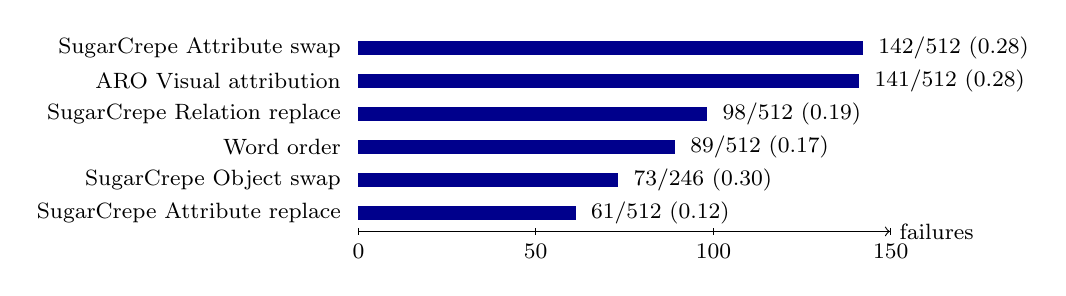
\begin{tikzpicture}[font=\footnotesize]
\node[anchor=east] at (-0.10,2.18) {SugarCrepe Attribute swap};
\draw[fill=blue!55!black,draw=blue!55!black] (0,2.10) rectangle (6.40,2.26);
\node[anchor=west] at (6.48,2.18) {142/512 (0.28)};
\node[anchor=east] at (-0.10,1.76) {ARO Visual attribution};
\draw[fill=blue!55!black,draw=blue!55!black] (0,1.68) rectangle (6.35,1.84);
\node[anchor=west] at (6.43,1.76) {141/512 (0.28)};
\node[anchor=east] at (-0.10,1.34) {SugarCrepe Relation replace};
\draw[fill=blue!55!black,draw=blue!55!black] (0,1.26) rectangle (4.42,1.42);
\node[anchor=west] at (4.50,1.34) {98/512 (0.19)};
\node[anchor=east] at (-0.10,0.92) {Word order};
\draw[fill=blue!55!black,draw=blue!55!black] (0,0.84) rectangle (4.01,1.00);
\node[anchor=west] at (4.09,0.92) {89/512 (0.17)};
\node[anchor=east] at (-0.10,0.50) {SugarCrepe Object swap};
\draw[fill=blue!55!black,draw=blue!55!black] (0,0.42) rectangle (3.29,0.58);
\node[anchor=west] at (3.37,0.50) {73/246 (0.30)};
\node[anchor=east] at (-0.10,0.08) {SugarCrepe Attribute replace};
\draw[fill=blue!55!black,draw=blue!55!black] (0,0.00) rectangle (2.75,0.16);
\node[anchor=west] at (2.83,0.08) {61/512 (0.12)};
\draw[->] (0,-0.15) -- (6.75,-0.15) node[right] {failures};
\draw (0.00,-0.11) -- (0.00,-0.19) node[below] {0};
\draw (2.25,-0.11) -- (2.25,-0.19) node[below] {50};
\draw (4.51,-0.11) -- (4.51,-0.19) node[below] {100};
\draw (6.76,-0.11) -- (6.76,-0.19) node[below] {150};
\end{tikzpicture}

    \caption{Largest remaining failure groups for the selected no-targeted, strong-anchor RRB model on the R030 diagnostic suite. The model still struggles with left/right spatial predicates, object and attribute swaps, and relation replacement cases.}
    \label{fig:failure_taxonomy}
\end{figure}
